\cleardoublepage

\chapter{Dream content}
\label{sec:dream-content}

\cleanchapterquote{Prétendre donner les rêves comme de simples jeux de la pensée, de simples images de l’imagination, c’est témoigner d’un manque de réflexion ou de loyauté ; car de toute évidence ils en diffèrent spécifiquement. Les images de l’imagination sont faibles, languissantes, incomplètes, partielles et si fugitives qu’on peut à peine fixer dans sa mémoire pendant quelques secondes les traits d’un absent, et que même le jeu le plus vif de l’imagination ne peut nullement entrer en comparaison avec la réalité palpable que le rêve met sous nos yeux.}{Schopenhauer}{Parerga und Paralipomena, 1851}

\section{Measuring dream content}
\label{sec:dream-content:method}

Empirical investigation of dreams started in the nineteenth century when scholars started to quantify aspects of their dream content. One notable example is the pioneering paper of Mary Calkins \citeyearpar{calkins_statistics_1893}, entitled \q{Statistics of dreams}, in which she reported, inter alia, statistics concerning dream length and vividness, dream characters and dream-waking-life associations. Since then, a considerable numbers of scales and rating systems for reducing and analyzing dream content have been developed, all based on the assumption that \q{particular aspects of the verbal material [..] have to be quantified in order to carry out statistical analyses} \citep{schredl_dream_2010}. Perhaps one of the most famous is the Hall \& Van de Castle coding system \citep{hall_content_1966}, whose basic idea is to divide dream content into several empirical categories (e.g. settings, objects, characters, interactions, emotions, misfortunes, and several others) that can be then used to find patterns and identify prevalent themes among groups of dreamers. The Hall \& Van de Castle coding system remains today the major reference since it has proven stable over at least one generation \citep{hall_dreams_1982}. More recently, \citet{schwartz_exploration_1999} proposed an automatic analysis of the lexical content of dream reports, without any a priori coding of their content, a method which has the advantage of minimizing the experimenter bias and being easily replicable by others.

As pointed out by \citet{schredl_dream_2010}, dream content analysis has several flaws. First, these scales, by reducing dream content to specific dimensions, voluntarily omit a certain amount of the information comprised within the dream report. Second, the results of these scales can drastically differ depending on whether the dream content is self-rated by the dreamer or rated by an external judge. As an example, \citet{sikka_i_2014} recently demonstrated that self-ratings resulted in higher scores of emotionality (i.e. greater estimates of (a) emotional dreams, (b) positively valenced dreams, (c) positive and negative emotions per dream, (d) and various discrete emotions).

\section{Phenomenology of dreams}
\label{sec:dream-content:pheno}

The empirical analyze of dream content using various scales has allowed to describe the following generalizations about the phenomenology of dreams (see also \citealp{hall_content_1966, schwartz_exploration_1999, schredl_characteristics_2010}):

\begin{my_list_item}
    \item Dreams tend to be negatively valenced
	\item Aggressions are more frequent in dreams than friendly interactions
	\item The visual modality is the predominant sensory modalities in dreams
	\item The dream drama is mostly lived by the dreamer from a first-person perspective
	\item Some elements of real-life events previously experienced by the dreamer often contribute to dream content
	\item Most of the time, the dream sequence is not within the dreamer’s voluntary control (i.e., the dreamer may be convinced during the dream that the dream’s story is really happening)
	\item Dream content often contains temporal and spatial inconsistencies
	\item Dream content is often full of people interacting with each other (e.g., discussions, fights, pursuit, sexuality)
	\item Dream content often contains intense emotions
\end{my_list_item}

\section{Factors influencing dream content}
\label{sec:dream-content:factors}

% First of all, gender differences in dream content have been consistently reported. According to some studies, men report more often physical aggression and sex than women \citep{nielsen_typical_2003, schredl_typical_2004}.

\paragraph{Cognitive organization}

As we mentioned earlier, there is ample evidence that waking experience finds its way into dreams. For instance, many aspects of the subject’s daily life influence dream content (reviewed in \citealp{ruby_experimental_2011}), including news event, musical practice, current concerns and religious beliefs, chronic pain, mood or living in a violent environment. However, the characteristics and time course of the waking memory sources integrated into dreams are still unclear. For instance, it is now well-admitted that dream content very rarely replays an episodic memory as it was originally experienced \citep{fosse_dreaming_2003, nielsen_what_2005}, although it is often related to some elements of the waking life of the dreamer \citep{schredl_characteristics_2010, blagrove_trait_2010, ruby_experimental_2011}. This observation has led to the so-called \q{continuity hypothesis of dreaming} which simply states that dreams reflect waking life experiences \citep{schredl_continuity_2003}.

Several factors have been positively associated with the likelihood of a waking life experience to be incorporated into dreams \citep{schredl_characteristics_2010}. These factors are reviewed in the following lines. First, there seems to be a linear decrease in temporal references identified in dreams, with recent experiences being more incorporated into dreams than older ones \citep{botman_dream_1990, strauch_dem_2004, grenier_temporal_2005}. This finding supports the notion of continuity between waking and dreaming memory processes. Furthermore, several studies \citep{botman_dream_1990, nielsen_day-residue_1992, marquardt_empirical_1996} have confirmed that a significant proportion of dreams contain elements that refer to experiences of the preceding day, a phenomenon known as day-residues and mentioned by Freud who considered them as \q{a necessary ingredient in dream formation} \citep{freud_interpretation_1900}. Another interesting finding is that contrary to what would be expected according to memory decay with time, some studies reported an overrepresentation in dreams of waking experiences that happened approximately one week before the dream \citep{nielsen_day-residue_1992, marquardt_empirical_1996, blagrove_replication_2011}, however this so-called \q{dream-lag effect} was not consistently found and seems to be specific to REM dreams \citep{blagrove_assessing_2011, van_rijn_dream-lag_2015}.
Second, several studies reported a preferential incorporation of emotional waking-life experiences into dreams \citep{malinowski_evidence_2014, schredl_factors_2006}. Interestingly, emotional intensity, but not emotional tone seems to affect the incorporation into subsequent dreams.
Third, all waking life activities are not represented in the same proportion in dreams \citep{hartmann_we_1996, schredl_continuity_2000}. Focused thinking activity (such as using a computer or reading) are rarely reported in dreams, an effect that might be explained by the generally low emotional intensity of these types of activities. Fourth, the magnitude of the continuity between waking and dreaming has been related to some extent to the personality traits of the dreamer \citep{schredl_dreaming_1996}. Finally, chronobiological factors, such as sleep cycles and time of the night, influence dream content. For example, dream reports from the first part of the night comprise more elements of the previous day than dream reports from the second part of the night \citep{roffwarg_effects_1978}.

\section{Dream construction}
\label{sec:dream-content:construction}

Based on these experimental findings, \citet{de_koninck_sleep_2012} has reviewed in his book entitled \q{Sleep, dreams and dreaming} the factors enabling dream construction, as well as their relative contribution to the dream content. He proposed that the different sources of dreams are best represented in a pyramidal manner, from low levels, predominant in shaping the dream content, to higher levels that carry much less influence to the dream content (Figure \ref{fig:intro:koninck}).

\begin{figure}[htb]
	\centering
	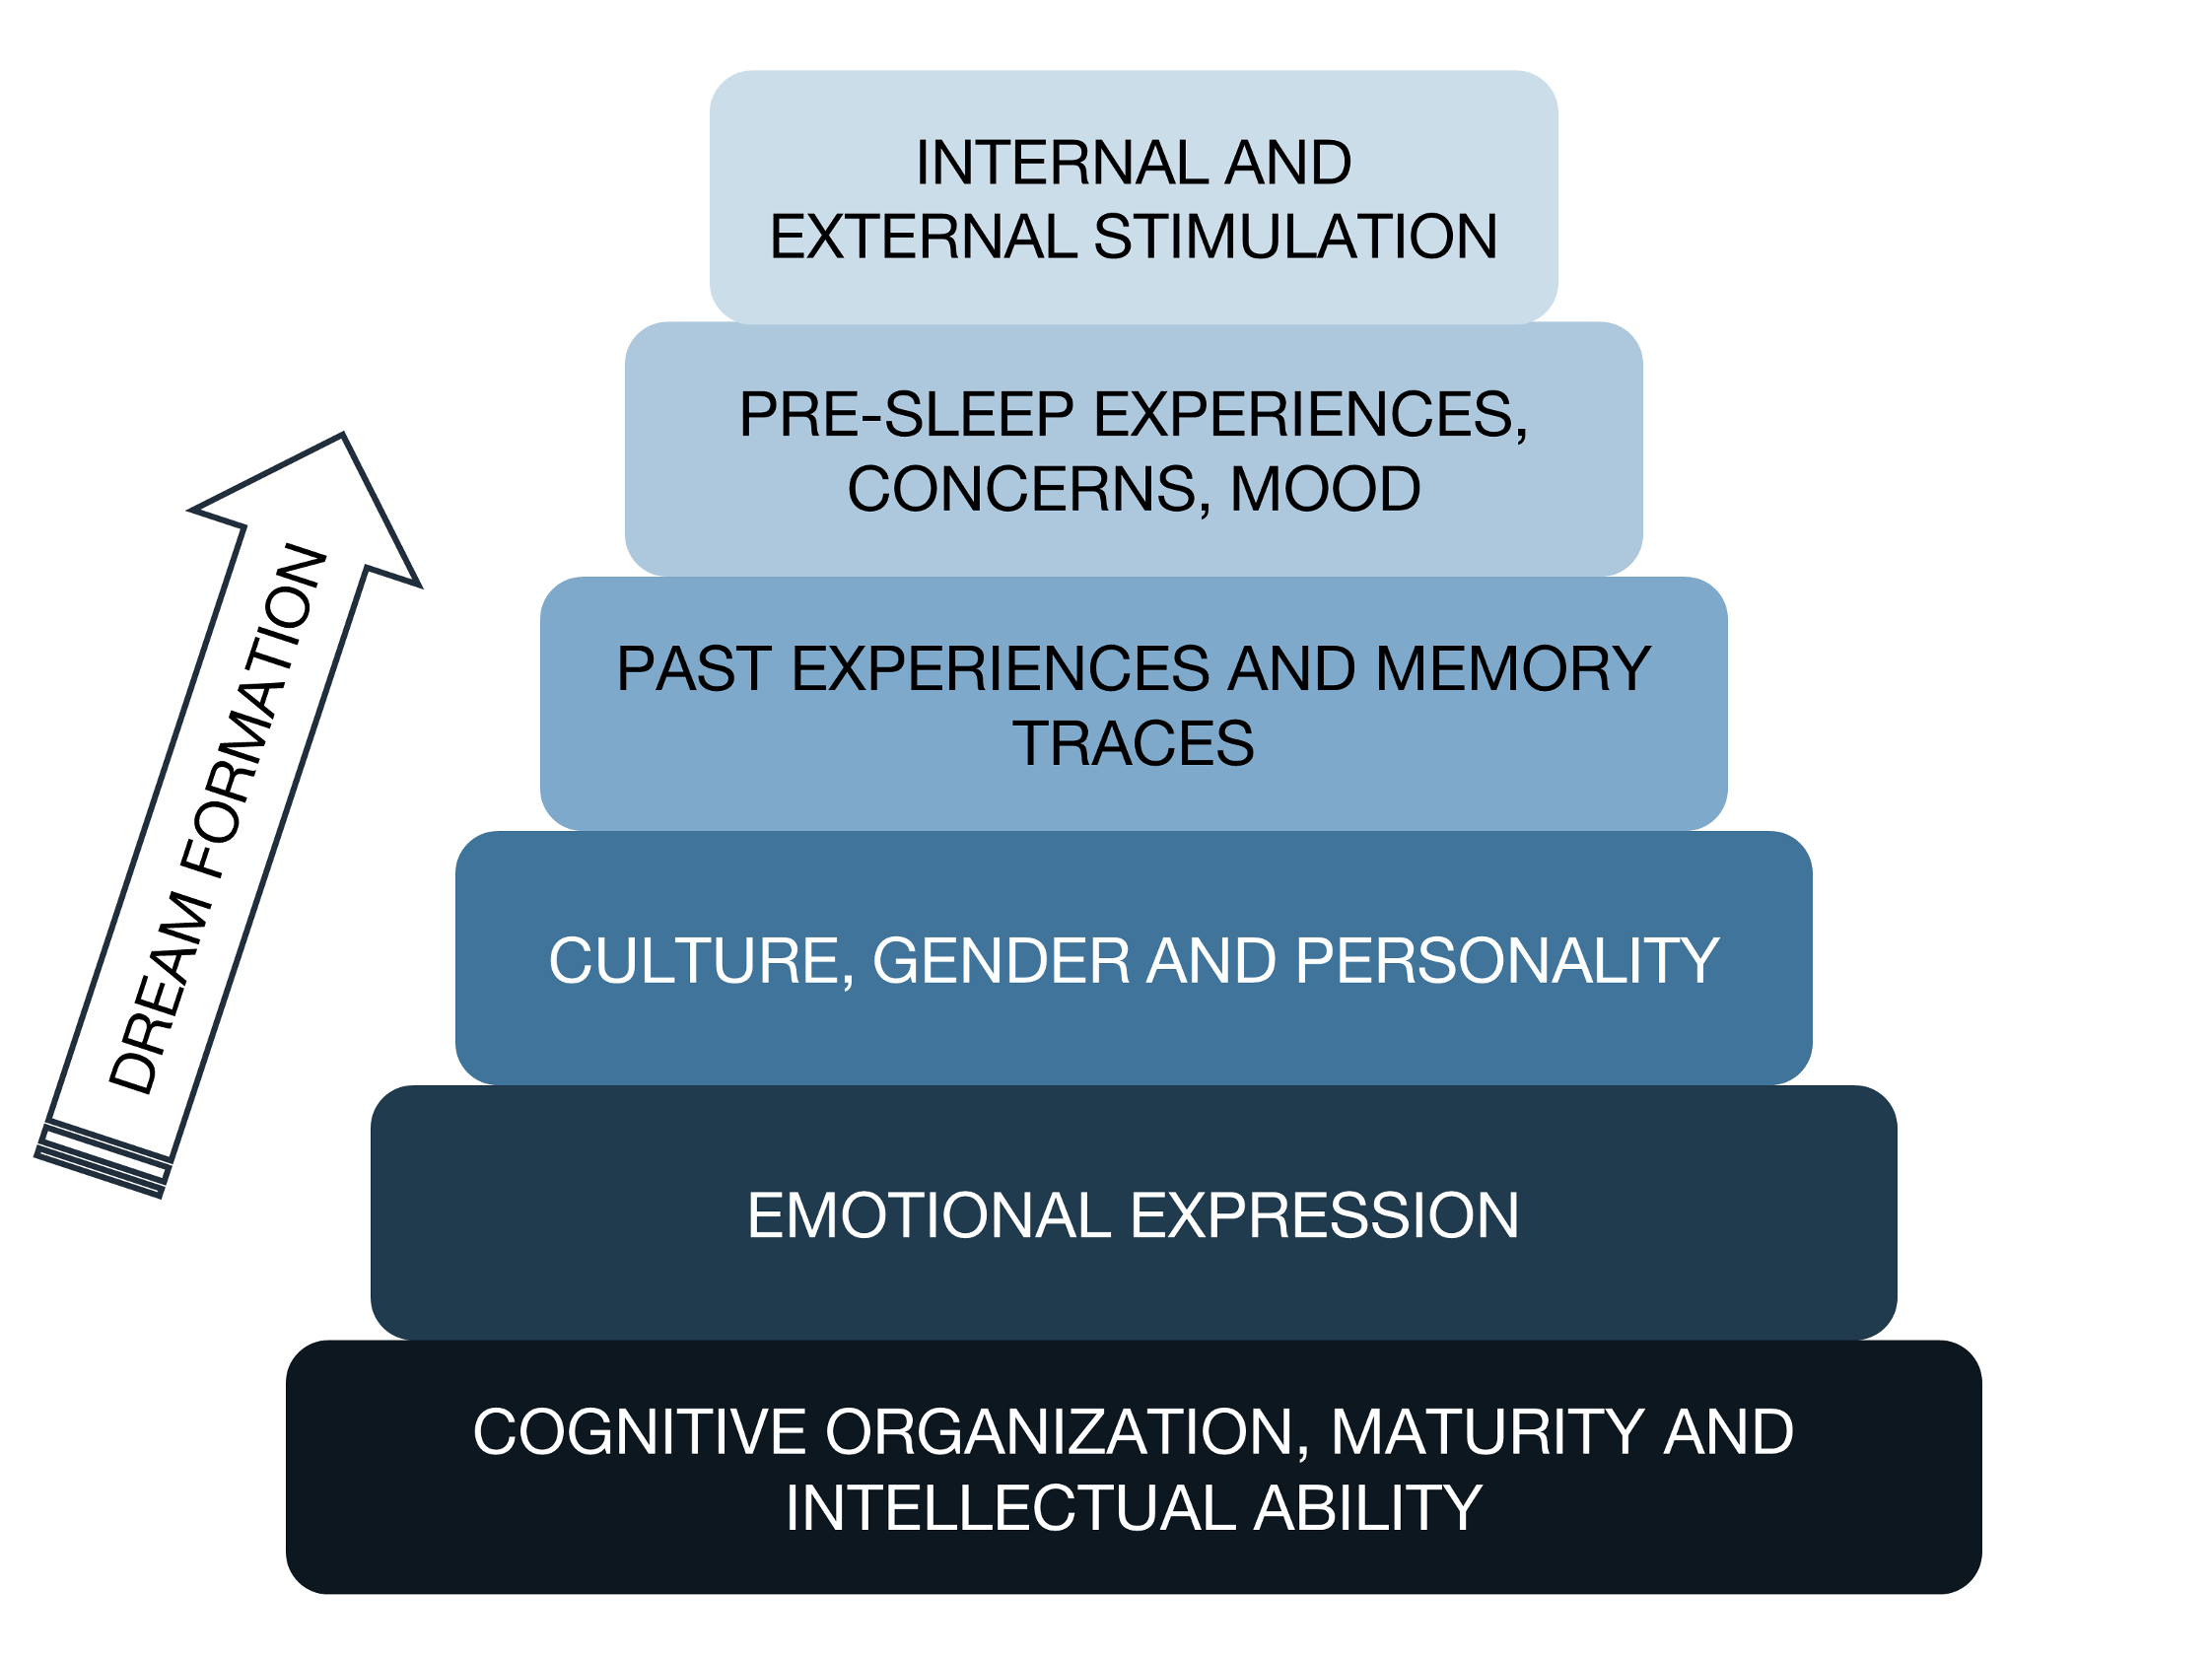
\includegraphics[width=0.75\textwidth]{Fig/Intro/Intro_Pyramid_dream_construction/Intro_pyramid_dream.png}
	\caption[Factors involved in the construction of dreams]{\textbf{Factors involved in the construction of dreams}. The various factors in the elaboration of dreaming are illustrated as a pyramid suggesting their order and importance. Adapted from \citet{de_koninck_sleep_2012}.}
	\label{fig:intro:koninck}
\end{figure}
